% % LLNCS macro package for Springer Computer Science proceedings;
% Version 2.21 of 2022/01/12
%
\documentclass[runningheads]{llncs}
%
\usepackage[T1]{fontenc}
% T1 fonts will be used to generate the final print and online PDFs,
% so please use T1 fonts in your manuscript whenever possible.
% Other font encondings may result in incorrect characters.
%

\usepackage{amsmath}
\usepackage{todonotes}

\usepackage[left=2cm,
            right=2cm,
            top=2cm,
            bottom=2cm]{geometry}

\usepackage{graphicx, color, float, subfig}
\captionsetup{font=small,labelfont=bf,labelsep=period,skip=5pt}
\captionsetup[subfloat]{font=scriptsize,labelfont=bf,skip=5pt}

%
\usepackage{hyperref}
\renewcommand\UrlFont{\color{blue}\rmfamily}
\urlstyle{rm}
%

\begin{document}
\title{\fontsize{12}{12}\selectfont Project 1 - Cat \& Dog Classification}
\titlerunning{Project 1}
%
\author{Henrik Daniel Christensen\orcidID{hench13@student.sdu.dk} \\Frode Engtoft Johansen\orcidID{fjoha21@student.sdu.dk}}
\authorrunning{Christensen, Johansen} % first names are abbreviated in the running head.
%
\institute{Deep Learning\\University of Southern Denmark, SDU\\\textit{Department of Mathematics and Computer Science}}
%
\maketitle % typeset the header of the contribution

%%%%%%%%%%%%%%%%%%%%%%%%%%%%%%%%%%%%%%%%%%%
\section{Introduction}
The objective of this project is to develop a deep learning model capable of distinguishing between images of cats and dogs.
The task involves training a neural network using a dataset containing 3,600 images, equally divided between the two categories.

% The report is structured as follows: Section 2 explores the dataset and the possible features that can be extracted from it.
% Section 3 describes which data augmentation techniques were used for the model training.
% Section 4 presents the architecture of the neural network.
% Section 5 describes the training process used to optimize the model.
% Section 6 presents the results obtained by the model.
% Section 7 presents the results of using a pre-trained model. Section 8 discusses the results and the limitations of the model.
% Finally, Section 9 concludes the report.
% In the Appendix, the code and a notebook with the results and visualizations are provided.
\section{Explorative Analysis}
\begin{figure}[H]
    \vspace*{-0.7cm}
    \centering
    \subfloat[][Cats]{%
        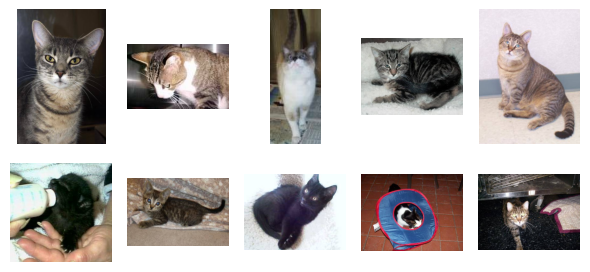
\includegraphics[width=0.35\textwidth]{figures/cats.png}\label{fig:cats}}\hspace{1cm}
    \subfloat[][Dogs]{%
        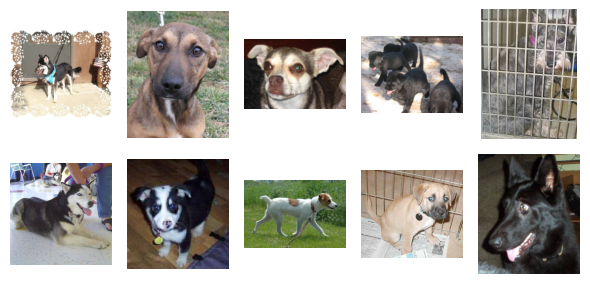
\includegraphics[width=0.35\textwidth]{figures/dogs.png}\label{fig:dogs}}
    \caption{Illustration of the effect of adaptive grids.}
    \label{fig:cats_dogs}
    \vspace*{-0.7cm}
\end{figure}

Dataset contains many diverse images and differ in terms of color, size, and orientation. The images are of varying quality, with some being clear and well-lit, while others are blurry or poorly framed. The dataset contains a mix of close-up shots and full-body shots of both cats and dogs. The dataset contains a mix of different breeds of cats and dogs, with varying fur lengths, colors, and patterns. Most of the pictures are 220-500 pixels wide, and 220-500 pixels tall. They are all in color, so they have 3 color channels. 

Cats vs. Dogs features
- Face:
- Cats generally have shorter, more rounded faces, often with triangular ears and pointed noses.
- Dogs generally have longer snouts and a greater diversity in ear shapes.
- Ears:
- Cats ears are typically upright and pointed.
- Dogs ears vary widely in shape and position, from erect to floppy, and they often have a different positioning on the head compared to cats.
- Eyes:
- Cats have generally more sharper-shaped eyes.
- Dogs have rounder eyes.
- Tail:
- Cats have long, flexible tails, often held upright or curled.
- Dogs’ tails vary greatly in length and shape, often held in different positions.
- Body Structure:
- Cats are generally lean, with flexible, agile bodies.
- Dogs come in a range of body types, from muscular to slender.
- Fur and Markings:
- Cats fur are often softer, finer, and smoother.
- Dogs often are coarser.
\section{Data Augmentation}
hej
\section{Model}
hej
\section{Training and Tuning}
\section{Results}
hej
\section{Pretrained model}
\section{Discussion}
\section{Conclusion}

\subsection{Individual Contributions}


%%%%%%%%%%%%%%%%%%%%%%%%%%%%%%%%%%%%%%%%%%%

%Appendices
\appendix
\section{Code}
hej
\includepdf[pages=1,scale=.85,pagecommand={\section{Notebook}\label{app:notebook}}]{../src/notebook.pdf}
\includepdf[pages=2-,scale=.85,pagecommand={}]{../src/notebook.pdf}

\bibliographystyle{base/splncs04}
\newpage
\bibliography{base/references}
%%%%%%%%%%%%%%%%%%%%%%%%%%%%%%%%%%%%%%%%%%%
\end{document}